\documentclass{rapportECL}
\addbibresource{biblio.bib}
\usepackage{booktabs}
\setlength\parskip{6pt}
\graphicspath{{figures/}}

\newcommand{\tok}[1]{\texttt{\small #1}}

\title{Rapport ECL - Qui utilise mon appli ?}

\begin{document}

%----------- Informations du rapport ---------

\titre{Qui utilise mon appli ? Identification des utilisateurs de Copilote}
\UE{MOD 7.2 -- Introduction à la science des données}
\sujet{BE -- Challenge Kaggle (groupe TD 4)}

\enseignant{
    Julien \textsc{Velcin}
}

\eleves{
    Seifeddine \textsc{Said} \\
    Souhaib \textsc{Zabi} \\
    Abdelhak \textsc{Tantaoui}
}

%----------- Initialisation -------------------
\fairepagedegarde
\fairemarges

%------------ Corps du rapport ----------------

\section{Introduction}

Copilote est un progiciel de gestion édité par Infologic et utilisé par des industriels de l'agro-alimentaire. Chaque utilisation du logiciel est enregistrée sous forme de session : le navigateur utilisé, puis la suite des actions réalisées (ouverture d'un écran, clic sur un bouton, saisie d'un champ, etc.).

L'objectif est de retrouver l'utilisateur qui a produit une session. C'est un problème de classification supervisée à 247 classes : l'utilisateur est connu pour les 3\,279 sessions d'entraînement et doit être prédit pour les 324 sessions de test. La principale difficulté est le faible nombre d'exemples par classe, une douzaine en moyenne. Le code est disponible sur \url{https://github.com/SeifSaid/be1} (notebook \tok{analyse.ipynb}).

\section{Données}

Chaque ligne contient l'identifiant de l'utilisateur (absent du test), le navigateur, puis les actions :

\begin{center}
\footnotesize\tok{nuh,Firefox,Création d'un écran(...AccueilController),t5,...}
\end{center}

Les jetons \tok{t5}, \tok{t10}, etc. sont des repères de temps : les actions qui précèdent \tok{t20} ont eu lieu dans les 20 premières secondes. Les sessions comptent de 0 à 11\,977 actions ; une lecture avec \tok{pandas.read\_csv} produirait plus de 14\,000 colonnes presque vides, sans signification commune d'une session à l'autre. Chaque ligne est donc lue comme une liste d'actions, puis chaque action est découpée par expressions régulières (tableau~\ref{tab:action}).

\begin{table}[!htbp]
\centering\small
\begin{tabular}{lll}
\toprule
Motif & Sens & Exemple \\
\midrule
texte avant \tok{(}, \tok{<} ou \tok{\$} & type d'action & \tok{Saisie dans un champ} \\
\tok{(...)} & écran & \tok{(...CRM\_ANNUAIRE.AnnuaireController)} \\
\tok{<...>} & configuration d'écran & \tok{<DEF\_03/24>} \\
\tok{\$...\$} & chaîne (catégorie de fiche) & \tok{\$GP\$} \\
\tok{1} final & fiche en modification & \tok{Saisie dans un champ1} \\
\bottomrule
\end{tabular}
\caption{Informations contenues dans une action}
\label{tab:action}
\end{table}

Pour les écrans, seule la fin du nom est conservée (\tok{AnnuaireController}). Aucune action ne se termine par un chiffre suivi d'un \tok{1}, ce qui rend la détection du mode modification sans ambiguïté. La simplification des noms regroupe en revanche 14 paires d'écrans distincts sur 426 (par exemple \tok{AvoirForm} pour les ventes et pour les achats) ; garder le nom complet ne change pas le score.

\section{Exploration des données}

\paragraph{Sessions par utilisateur.} Les utilisateurs ont entre 4 et 75 sessions, avec une médiane de 12 (figure~\ref{fig:explo}). Prédire toujours l'utilisateur le plus fréquent donne 2,3~\% de bonnes réponses, le hasard 0,4~\%. Certaines classes doivent être apprises à partir de 3 sessions, et la validation doit tenir compte de ces classes rares.

\paragraph{Navigateur.} Chacun des 247 utilisateurs n'utilise qu'un seul navigateur : Firefox (114 utilisateurs), Chrome (93), Edge (39) ou Opera (1). La répartition est la même dans le train et le test. Une session Edge ne peut donc venir que d'un des 39 utilisateurs d'Edge (partie~\ref{sec:nav}).

\paragraph{Longueur des sessions.} La distribution est très asymétrique : médiane de 340 actions (environ 6 minutes), maximum de 11\,977 actions (plus de 3 heures). Toutes les sessions sont conservées : ce sont des sessions réelles, le test en contient de semblables, certains utilisateurs n'en ont que 4, et la normalisation TF-IDF empêche une session longue de peser davantage qu'une autre.

\paragraph{Types d'action.} Il n'existe que 35 types d'action, et les plus courants (exécution d'un bouton, affichage d'une dialogue, saisie dans un champ) apparaissent dans presque toutes les sessions. Il faut donc réduire leur poids et utiliser aussi les écrans, configurations et chaînes.

\paragraph{Similarité entre sessions.} En représentant chaque session par la fréquence de ses types d'action, la similarité cosinus médiane vaut 0,88 entre deux sessions du même utilisateur, contre 0,56 entre deux utilisateurs différents (figure~\ref{fig:explo}). Chaque utilisateur a une façon de travailler reconnaissable, mais les deux distributions se recouvrent : les types d'action seuls ne suffiront pas.

\begin{figure}[!htbp]
\centering
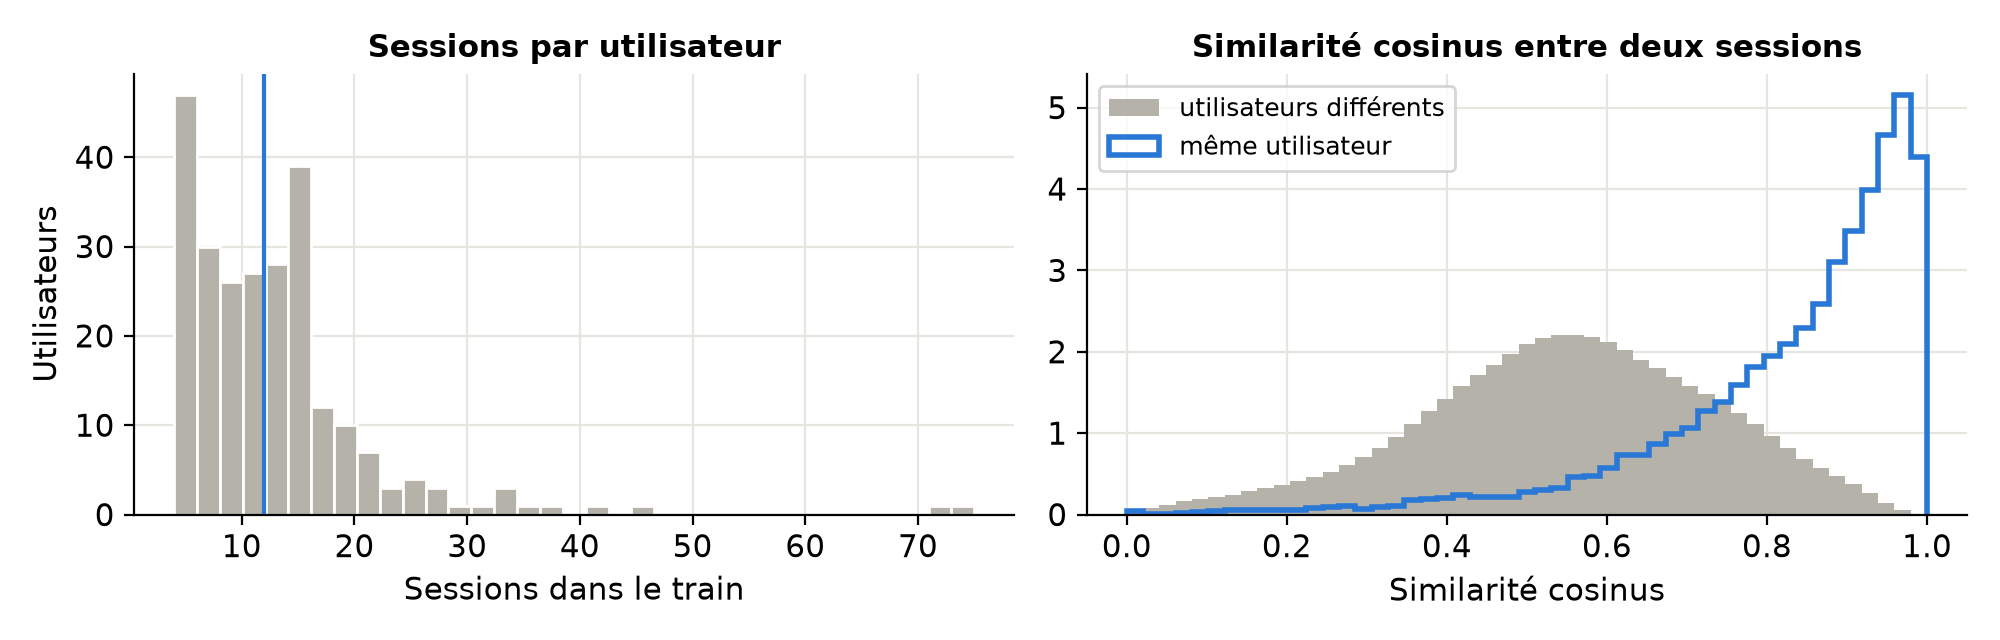
\includegraphics[width=\linewidth]{exploration.png}
\caption{Nombre de sessions par utilisateur (médiane en bleu) et similarité cosinus entre paires de sessions, calculée sur les profils de types d'action}
\label{fig:explo}
\end{figure}

\section{Représentation des sessions}
\label{sec:repr}

Chaque session est traitée comme un document dont les actions sont les mots, ce qui permet d'utiliser les méthodes de classification de textes. Chaque action produit son type, puis éventuellement \tok{ECRAN\_...}, \tok{CONF\_...}, \tok{CHAINE\_...} et \tok{MODIF} ; le navigateur est ajouté en début de session (\tok{NAV\_Firefox}). Ce texte est vectorisé par TF-IDF : le logarithme du nombre d'occurrences (\tok{sublinear\_tf}) limite le poids des actions répétées, l'IDF réduit celui des mots présents partout, et la normalisation rend comparables des sessions de longueurs très différentes. Les bigrammes conservent une partie de l'ordre : un bigramme est soit une transition entre deux actions (\tok{Raccourci Exécution\_d\_un\_bouton}), soit une action associée à son écran (\tok{Raccourci ECRAN\_SaisiEcritForm}). Les mots présents dans une seule session sont ignorés ; le vocabulaire compte 9\,002 mots, dont 8\,400 bigrammes.

À titre de comparaison, nous avons aussi résumé chaque session par 43 variables : nombre d'actions, durée, nombre de types et d'écrans distincts, navigateur (encodage one-hot) et proportion de chaque type d'action.

\section{Protocole d'évaluation}

Nous utilisons une validation croisée stratifiée à 4 plis. Le nombre de plis est imposé par l'utilisateur le plus rare (4 sessions) : chaque pli de test contient une de ses sessions et l'entraînement en garde trois. Le vectoriseur TF-IDF est placé dans un \tok{Pipeline} avec le modèle, donc recalculé à chaque pli sur les seules sessions d'entraînement, ce qui évite toute fuite de données.

Deux métriques sont suivies : l'accuracy, proportion de sessions attribuées au bon utilisateur, et le F1 macro, moyenne sur les 247 utilisateurs du F1-score de chaque utilisateur, qui donne le même poids aux utilisateurs rares et fréquents. L'écart-type de l'accuracy entre les plis (environ 0,6 point) sert de référence pour juger si une différence est significative ; les choix importants sont vérifiés sur trois découpages différents.

\section{Modèles et résultats}

\subsection{Comparaison des modèles}

\begin{table}[!htbp]
\centering\small
\begin{tabular}{lccc}
\toprule
Modèle & Accuracy & F1 macro & Entraînement \\
\midrule
Classe majoritaire & 2,3~\% $\pm$ 0,1 & 0,0~\% & -- \\
Forêt aléatoire (43 variables) & 85,1~\% $\pm$ 2,0 & 81,9~\% & 10,5 s \\
Plus proche voisin (TF-IDF) & 89,4~\% $\pm$ 1,2 & 87,6~\% & 2,5 s \\
Régression logistique (TF-IDF, $C = 10$) & 93,3~\% $\pm$ 0,6 & 90,5~\% & 26,0 s \\
SVM linéaire (TF-IDF, $C = 0{,}5$) & 94,7~\% $\pm$ 0,8 & 92,7~\% & 5,2 s \\
\bottomrule
\end{tabular}
\caption{Comparaison des modèles avant réglage, sur le texte simple (validation croisée à 4 plis)}
\label{tab:modeles}
\end{table}

La forêt aléatoire (tableau~\ref{tab:modeles}) ne voit ni les écrans ni les chaînes, ce qui explique au moins en partie son retard. Le plus proche voisin s'appuie sur une seule session et reste sensible au bruit. Les modèles linéaires sur TF-IDF sont les meilleurs : avec 9\,000 variables pour une douzaine d'exemples par classe, les classes sont presque toujours séparables linéairement, un modèle plus complexe aurait tendance à surapprendre, et les vecteurs creux sont traités efficacement. Le SVM, qui maximise la marge entre chaque utilisateur et les autres (un contre tous), obtient le meilleur score et s'entraîne 5 fois plus vite que la régression logistique.

\subsection{Apport de chaque information}

\begin{table}[!htbp]
\centering\small
\begin{tabular}{lcc}
\toprule
 & Sans bigrammes & Avec bigrammes \\
\midrule
Types d'action seuls & 59,4~\% & 84,7~\% \\
+ écrans, configurations, chaînes & 85,3~\% & 94,1~\% \\
+ écrans, configurations, chaînes + navigateur & -- & 94,7~\% \\
\bottomrule
\end{tabular}
\caption{Accuracy selon les informations utilisées (SVM linéaire, $C = 0{,}5$, texte simple)}
\label{tab:ablation}
\end{table}

Les types d'action seuls donnent 59~\% (tableau~\ref{tab:ablation}). Les bigrammes et les écrans apportent chacun autant (environ 85~\%), et le gain attribué à chacun dépend de l'ordre dans lequel on les ajoute. Combinés, ils gagnent encore 9 points : ils sont complémentaires, les bigrammes décrivant la façon dont l'utilisateur enchaîne ses actions et les écrans ce sur quoi il travaille. Ajouté comme un simple mot, le navigateur n'apporte que 0,6 point.

\subsection{Réglage des hyperparamètres}

Le paramètre $C$ du SVM règle le compromis entre sous-apprentissage ($C$ petit) et surapprentissage ($C$ grand). Avec une validation croisée répétée trois fois (12 entraînements par valeur), l'accuracy passe de 88,3~\% pour $C = 0{,}1$ à 96,0~\% pour $C = 3$, puis atteint un plateau (96,1~\% pour $C = 10$ et $C = 30$, des écarts inférieurs à l'écart-type). Nous retenons $C = 10$. Réglée de la même façon, la régression logistique atteint au mieux 94,7~\% ($C = 100$), contre 96,2~\% pour le SVM sur les mêmes plis : le SVM est retenu.

\subsection{Le navigateur comme contrainte}
\label{sec:nav}

Le SVM réglé fait 125 erreurs, dont 61 désignent un utilisateur qui n'utilise pas le navigateur de la session : le navigateur n'est qu'un mot parmi 9\,000 et pèse très peu. Nous appliquons donc directement la règle observée pendant l'exploration : pour chaque session, le SVM donne un score à chacun des 247 utilisateurs (\tok{decision\_function}), les utilisateurs d'un autre navigateur reçoivent un score de $-\infty$, et on retient le meilleur score restant. Cette règle n'introduit pas de fuite : chaque utilisateur a au moins trois sessions dans l'entraînement de chaque pli, toutes avec le même navigateur. Elle échouerait seulement si un utilisateur changeait de navigateur, ce qui n'arrive jamais dans le train. L'accuracy passe de 96,2~\% à 97,2~\% (tableau~\ref{tab:evolution}), et ce gain se retrouve sur les trois découpages.

\begin{table}[!htbp]
\centering\small
\begin{tabular}{lcc}
\toprule
Modèle (SVM linéaire, $C = 10$) & Accuracy (moyenne sur 3 découpages) & F1 macro \\
\midrule
Texte simple & 96,2~\% & 95,8~\% \\
Texte simple + contrainte du navigateur & \textbf{97,2~\%} & \textbf{96,9~\%} \\
\bottomrule
\end{tabular}
\caption{Effet de la contrainte du navigateur (F1 macro calculé sur le premier découpage)}
\label{tab:evolution}
\end{table}

\subsection{Pistes sans effet}

Trois autres idées ont été testées sur les mêmes plis, à partir du SVM réglé (96,2~\%) : les trigrammes (96,2~\%, pour un temps d'entraînement doublé), un poids plus élevé pour les utilisateurs rares avec \tok{class\_weight="balanced"} (96,3~\%), et la conservation des repères de temps comme mots pour capter le rythme de travail (96,4~\%). Ces écarts sont inférieurs à l'écart-type entre plis (0,6 point) : le modèle reste dans sa version la plus simple.

\section{Analyse des erreurs et interprétation}

\subsection{Erreurs du modèle final}

Le modèle final (SVM et contrainte du navigateur) fait 93 erreurs sur 3\,279 sessions sur le premier découpage (figure~\ref{fig:erreurs}). Les sessions courtes sont les plus difficiles (92,5~\% pour le quart le plus court, 99,6~\% pour le plus long), car elles contiennent peu d'indices. Le nombre de sessions de l'utilisateur compte peu : 96,3~\% de 4 à 7 sessions, 96,4~\% de 8 à 15, 98,1~\% au-delà ; sans la contrainte, l'écart était plus marqué, car une partie des erreurs sur les utilisateurs rares venait d'un mauvais navigateur. Le bon utilisateur figure parmi les trois premiers choix pour 99,1~\% des sessions, et les erreurs se concentrent sur quelques paires : \tok{skm} et \tok{slq} (7 erreurs), \tok{flj} et \tok{skm} (6), puis trois paires à 3 erreurs. Comme $C$ a été choisi sur ces mêmes plis, ce score est légèrement optimiste ; le score Kaggle en donne une mesure indépendante.

\begin{figure}[!htbp]
\centering
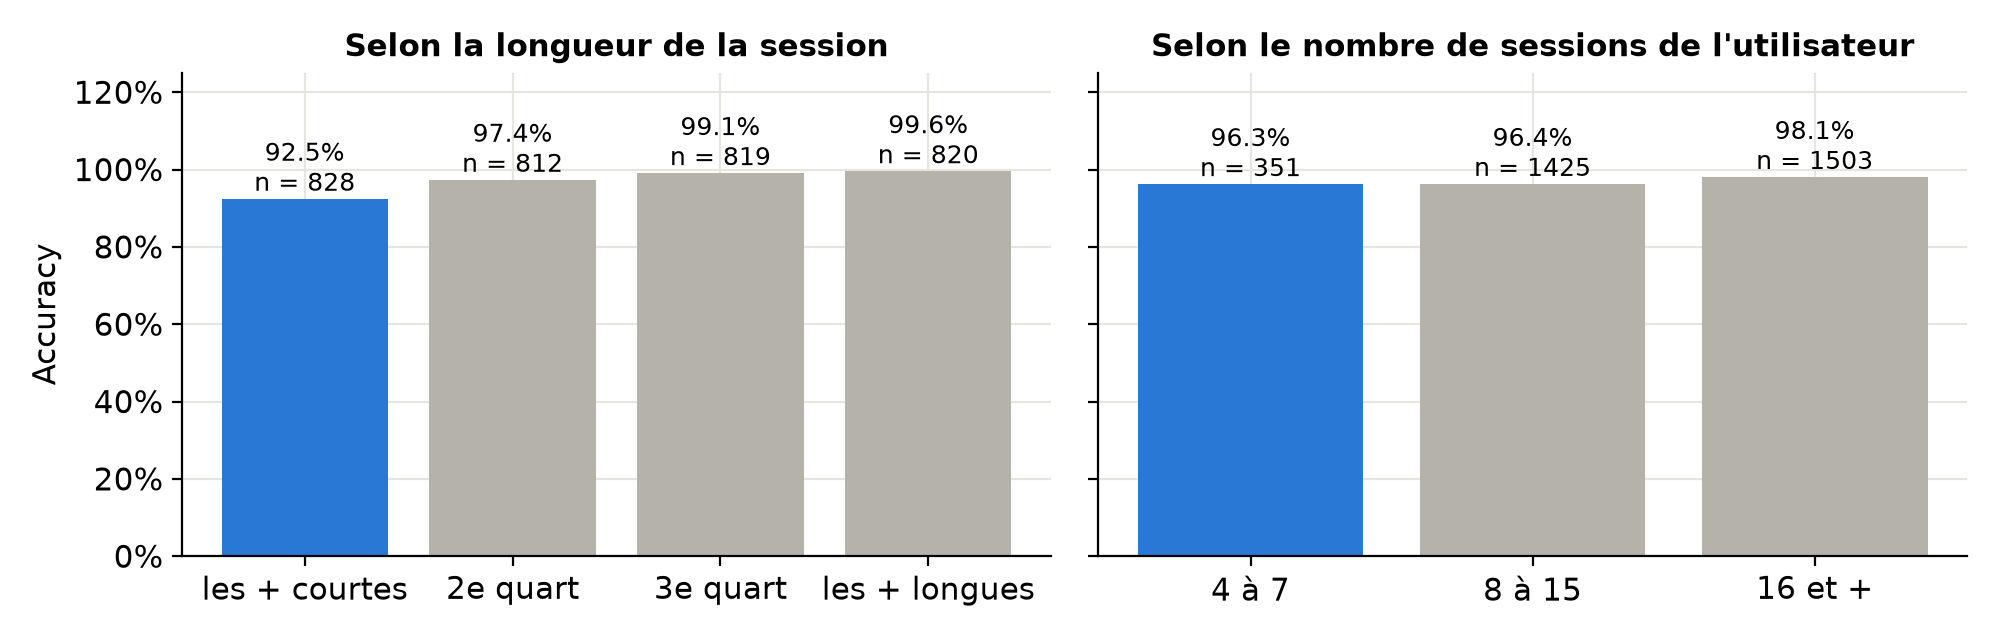
\includegraphics[width=\linewidth]{erreurs.png}
\caption{Accuracy du modèle final selon la longueur de la session (quarts) et selon le nombre de sessions de l'utilisateur ($n$ : nombre de sessions du groupe)}
\label{fig:erreurs}
\end{figure}

\subsection{Variables les plus influentes}

Le SVM apprend un poids par mot et par utilisateur. Nous mesurons la contribution d'un mot par la somme des valeurs absolues de ses poids sur les 247 utilisateurs, multipliée par sa valeur moyenne. Le poids seul serait trompeur : un mot présent partout, comme \tok{NAV\_Firefox}, a une valeur TF-IDF très faible et a besoin d'un grand poids pour compter.

\begin{table}[!htbp]
\centering\small
\begin{tabular}{lrr}
\toprule
Famille de mots & Nombre de mots & Contribution \\
\midrule
Bigrammes d'actions & 984 & 44~\% \\
Bigrammes avec écran, configuration ou chaîne & 7\,416 & 29~\% \\
Types d'action & 35 & 14~\% \\
Écrans & 296 & 7~\% \\
Configurations & 198 & 3~\% \\
Chaînes & 68 & 2~\% \\
Modification (\tok{MODIF}) & 1 & 1~\% \\
Navigateur & 4 & 1~\% \\
\bottomrule
\end{tabular}
\caption{Contribution de chaque famille de mots au modèle final}
\label{tab:familles}
\end{table}

Les transitions entre actions ont la contribution la plus forte (tableau~\ref{tab:familles}) : l'enchaînement des actions est ce qui distingue le plus les utilisateurs. Viennent ensuite les bigrammes associant une action à un écran ou une configuration, puis les écrans, ce qui rejoint la complémentarité observée dans l'ablation. Le navigateur ne contribue presque pas, ce qui explique l'efficacité de la contrainte. À l'échelle d'un utilisateur, les mots de plus fort poids forment une signature : \tok{skm} utilise les raccourcis clavier sur l'écran de saisie d'écritures comptables (\tok{Raccourci ECRAN\_SaisiEcritForm}) avec la configuration \tok{CONF\_ADM\_055}, et \tok{slq} travaille aussi sur cet écran, ce qui explique leurs confusions ; \tok{cjr} travaille sur des formulaires et comptes rendus avec la configuration \tok{CONF\_SuiviProdLog}, liée au suivi de production.

\section{Résultats sur Kaggle}

Le modèle final est entraîné sur les 3\,279 sessions du train puis appliqué aux 324 sessions de test. La contrainte du navigateur modifie 4 prédictions, et les 2 sessions sous Opera sont attribuées à \tok{swe}, unique utilisateur de ce navigateur.

\begin{table}[!htbp]
\centering\small
\begin{tabular}{lccc}
\toprule
Soumission & Accuracy (CV) & F1 macro (CV) & Kaggle \\
\midrule
v1 : SVM seul & 96,2~\% & 95,8~\% & 0,963 \\
v2 : SVM + contrainte du navigateur & 97,2~\% & 96,9~\% & 0,982 \\
\bottomrule
\end{tabular}
\caption{Scores en validation croisée et sur Kaggle}
\label{tab:kaggle}
\end{table}

Les scores Kaggle sont proches des scores de validation croisée, ce qui confirme que le protocole n'était pas biaisé. Sur 324 sessions, aucun nombre de bonnes réponses ne donne exactement 0,982 (318 donnent 0,981 et 319 donnent 0,985) : le score Kaggle n'est donc pas une accuracy simple, plus probablement une F-mesure moyenne sur les utilisateurs, et ne se compare qu'approximativement aux scores de validation croisée. La contrainte du navigateur se confirme nettement : elle ne modifie que 4 prédictions mais fait gagner 0,019. Avec seulement 324 sessions de test, une seule prédiction changée peut déplacer le score de quelques millièmes : les écarts de cet ordre au classement ne sont pas significatifs.

\section{Conclusion}

En représentant chaque session comme un texte pondéré par TF-IDF, un SVM linéaire identifie l'utilisateur parmi 247 avec 97,2~\% d'accuracy en validation croisée, une fois appliquée la contrainte du navigateur tirée de l'exploration. Les utilisateurs se distinguent à la fois par l'enchaînement de leurs actions et par les écrans sur lesquels ils travaillent. Les erreurs restantes concernent surtout les sessions courtes et des utilisateurs qui travaillent sur les mêmes écrans.

Deux limites demeurent : le score de validation est légèrement optimiste car $C$ a été choisi sur les mêmes plis, et la contrainte suppose qu'un utilisateur ne change pas de navigateur. Par ailleurs, le test ne compte que 324 sessions : un gain de l'ordre d'une session ne peut pas y être vérifié.

\begin{thebibliography}{99}

\bibitem{Salton1988}
G. Salton et C. Buckley. \emph{Term-weighting approaches in automatic text retrieval}. Information Processing \& Management, 24(5):513--523, 1988.

\bibitem{Cortes1995}
C. Cortes et V. Vapnik. \emph{Support-vector networks}. Machine Learning, 20(3):273--297, 1995.

\bibitem{Joachims1998}
T. Joachims. \emph{Text categorization with Support Vector Machines: learning with many relevant features}. European Conference on Machine Learning (ECML), 1998.

\bibitem{Pedregosa2011}
F. Pedregosa et al. \emph{Scikit-learn: Machine Learning in Python}. Journal of Machine Learning Research, 12:2825--2830, 2011.

\bibitem{Kaggle}
Kaggle, \emph{Qui utilise mon appli ? Challenge}.\\ \url{https://www.kaggle.com/competitions/qui-utilise-mon-appli-challenge/}

\end{thebibliography}
\end{document}
